The user interface is composed of one web-page developed in HTML 5 with some
pieces of JavaScript and CSS \footnote{\url{https://github.com/ProjetPP/PPP-WebUI/}}.
We have taken care of having an
interface that fits nice on both huge screens of desktop computers
and small screens of phones using responsive design techniques.

\begin{figure}[!ht]
    \centering
    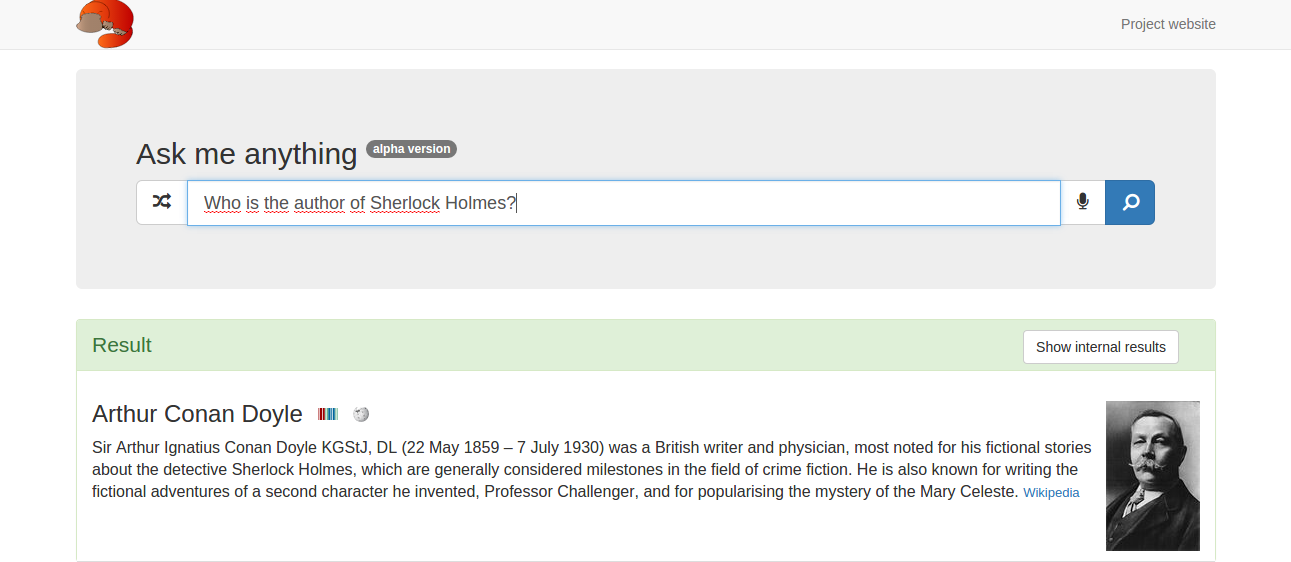
\includegraphics[width=1\textwidth]{WebUI.png}
    \caption{The user interface (Wikipedia header)}
\end{figure}

\begin{figure}[!ht]
    \centering
    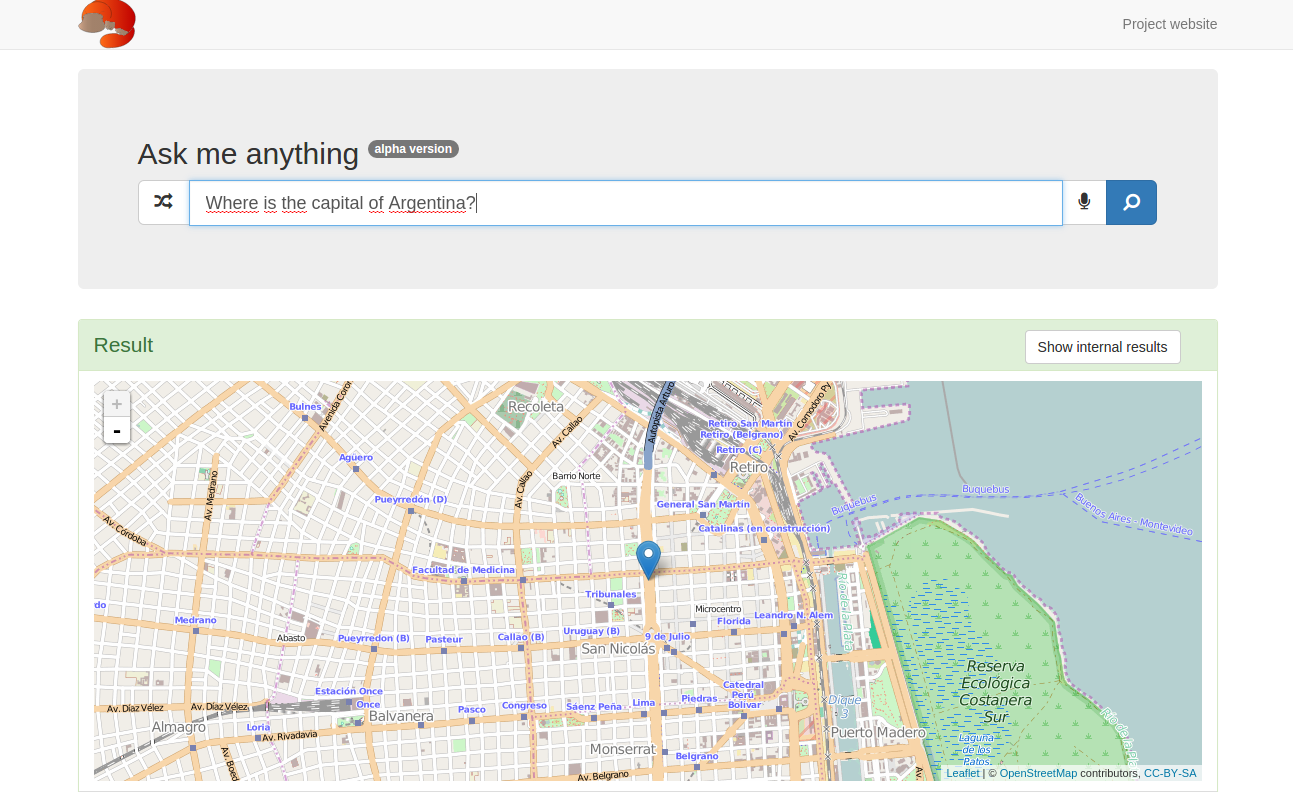
\includegraphics[width=1\textwidth]{WebUI2.png}
    \caption{The user interface (OpenStreetMap location)}
\end{figure}

It is made of one huge text input with a button to submit
the query and another one to get a random question from a hand written list. The text area
allows to input question in natural language or using the data model notation like
\texttt{(Douglas Adam, birth date,?)} to find the
birth date of Douglas \textsc{Adam}. A parser written as a Python module
\footnote{\url{https://github.com/ProjetPP/PPP-datamodel-Python/blob/master/ppp\_datamodel/parsers.py}}
using
the PLY\footnote{\url{http://www.dabeaz.com/ply/}} library converts
the data model notation into the internal JSON representation.

In order to build this interface we have relied on some famous libraries 
like jQuery\footnote{\url{http://jquery.com/}}, Bootstrap\footnote{\url{http://getbootstrap.com}}, MathJax\footnote{\url{http://www.mathjax.org/}} to display mathematics and Leaflet\footnote{\url{http://leafletjs.com/}} for maps.

\section{Logging}

All requests send to the PPP are logged to improve our algorithms
and particularly to feed the results to Question parsing
modules that use Machine Learning.
We may also use it to improve the way the Core routes and sorts answers
from the different modules, either manually or with some basic
Machine Learning.

The main idea is to log user feedback in addition to the requests
themselves: after showing the user the way we interpreted their
question alongside the answer to their request, we provide them a
way to give us feedback.
What we call feedback is actually a thumb up / thumb down pair of
buttons, and, if the latter is pressed, a way to correct the requests
parsing result so it can be fed to the Machine Learning algorithms.

Since Machine Learning algorithms are not ready yet, we did not focus
on this feature of the user interface and thus it is not implemented yet;
so far we only started implemented a backend that stores data
(gathered via the user interface) to a SQLite database.
This already provides us a database of questions asked by people
outside the project.
